% --- CORRESPONDE A: conclusiones.tex ---
% --- DIAPOSITIVA 25: CONCLUSIONES (II) - PRINCIPALES LOGROS ---
\begin{frame}{Conclusiones: Principales Logros}
	\footnotesize
	\begin{itemize}
		\item Estudio del marco teórico matricial para Polinomios Ortogonales de Sobolev.
		\item Validación numérica de condiciones de acotación de $\mathcal{D}$ en diversos contextos geométricos.
		\item Análisis pionero del comportamiento de $\sigma_{2,n}$ en operadores no secuencialmente dominados.
		\item Implementación de algoritmos eficientes en \textsc{Maple}.
		\item Creación de un sistema interactivo de visualización.
		\item Desarrollo personal.
	\end{itemize}
\end{frame}

% --- CORRESPONDE A: conclusiones.tex ---
% --- DIAPOSITIVA 28: LÍNEAS DE TRABAJO FUTURO (I) ---
\begin{frame}{Líneas de Trabajo Futuro (I)}
	\footnotesize
	Se abren diversos frentes de investigación:
	\begin{itemize}
		\item \textbf{Productos Sobolev de orden superior ($N>1$):}
		      \begin{itemize}
			      \item Incorporar derivadas de segundo y tercer orden.
			      \item Analizar valores singulares siguientes ($\sigma_{3,n}, \sigma_{4,n},...$).
		      \end{itemize}
		      \pause
		\item \textbf{Leyes de distribución de ceros:}
		      \begin{itemize}
			      \item Derivar distribuciones límite (tipo medida de equilibrio) para los ceros en distintos regímenes (analogía con Ullman-Stahl).
		      \end{itemize}
		      \pause
		\item \textbf{Convergencia del autovalor máximo:}
		      \begin{itemize}
			      \item Investigar si el autovalor que determina $\rho(\mathbf{D}_n)$ converge.
		      \end{itemize}
	\end{itemize}
\end{frame}

% --- DIAPOSITIVA 30: LÍNEAS DE TRABAJO FUTURO (III) - EJEMPLOS CON DERIVADAS DE ORDEN SUPERIOR ---
\begin{frame}{Líneas de Trabajo Futuro (II) - Ejemplos con Derivadas de Orden Superior}
	\footnotesize
	\begin{columns}[T]
		\begin{column}{0.48\textwidth}
			\textbf{Ejemplo 1:}
			\tiny
			$\langle p,q \rangle_{S}=\int_{0}^{10} pq\, dt + \int_{30}^{40} p'q' \, dt + \int_{60}^{70} p''q'' \, dt$

			\vspace{-0.3em}
			\begin{figure}
				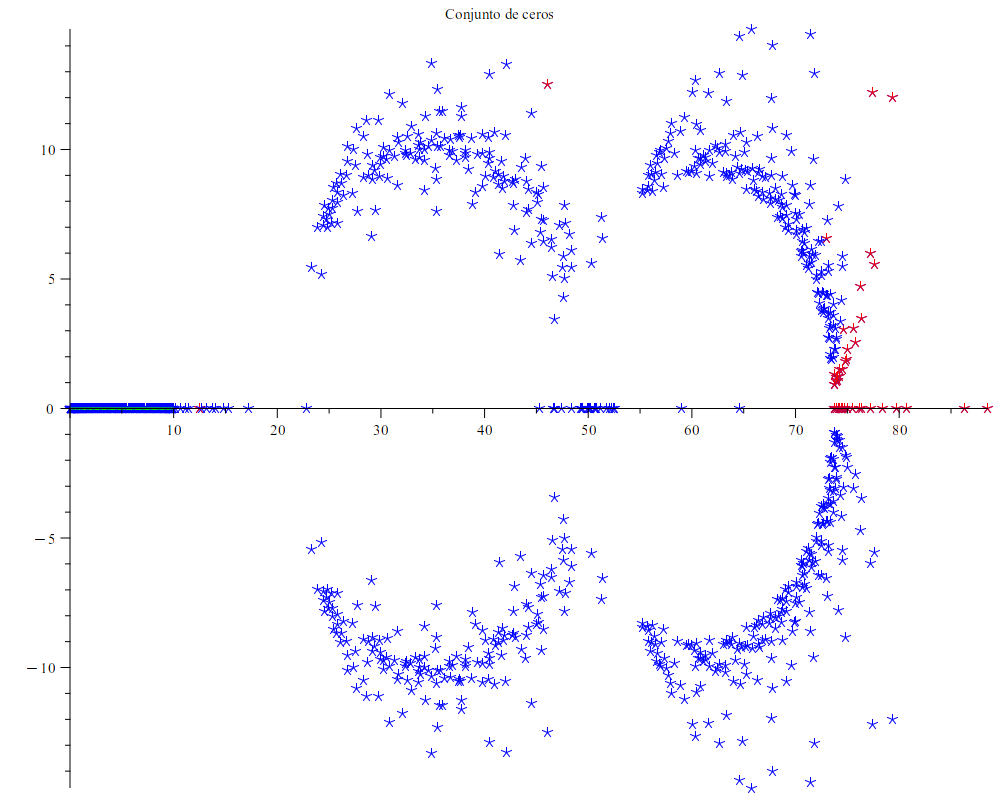
\includegraphics[width=0.8\linewidth]{tfg_latex_etsiinf-2023.02.20/include/a0b10c30d40e60f70_zeros.png}
			\end{figure}
			\vspace{-1.5em}

			\textbf{Datos ($n=70$):}
			\begin{itemize}
				\item $\sigma_{1,70} \approx 4.94 \times 10^{8}$
				\item $\sigma_{2,70} \approx 1.85 \times 10^{8}$
				\item $\sigma_{3,70} \approx 69.956$
				\item $R = 70$
				\item $\rho(\mathbf{D}_{70}) \approx 73.791$
			\end{itemize}
		\end{column}

		\begin{column}{0.48\textwidth}
			\textbf{Ejemplo 2:}
			\tiny
			$\langle p,q \rangle_{S}=\int_{0}^{10} pq\, dt + \int_{30}^{40} p'q' \, dt + p''(0)q''(0)$

			\vspace{-0.3em}
			\begin{figure}
				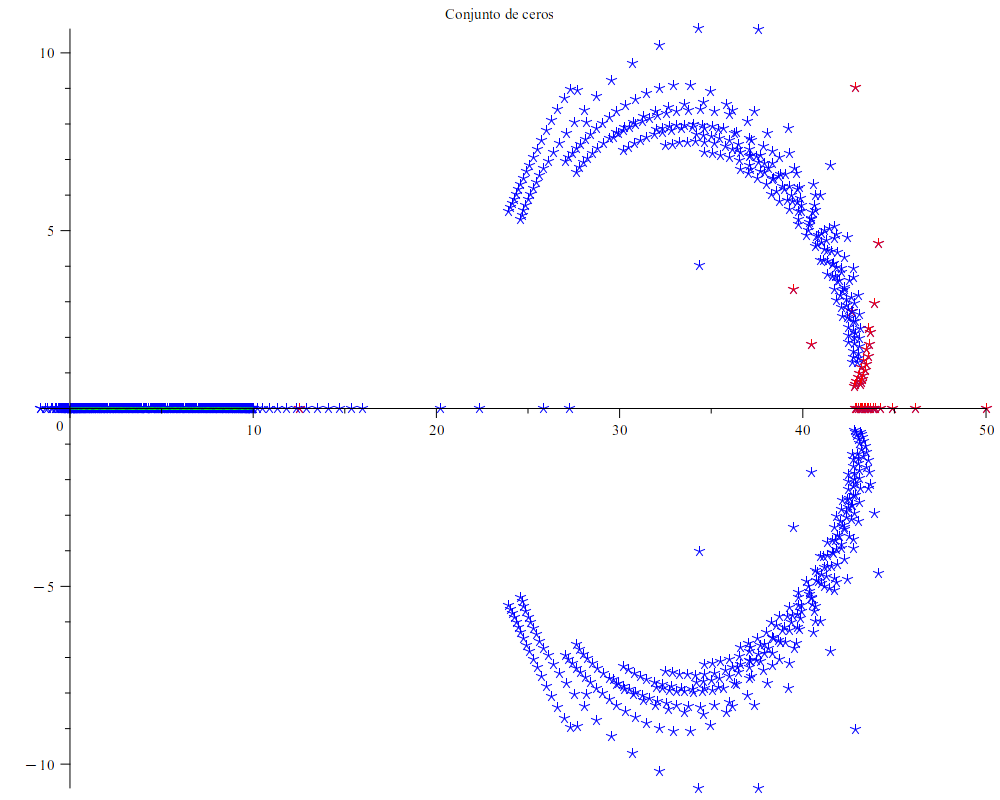
\includegraphics[width=0.8\linewidth]{tfg_latex_etsiinf-2023.02.20/include/a0b10c30d40t0_zeros.png}
			\end{figure}
			\vspace{-1.5em}

			\textbf{Datos ($n=70$):}
			\begin{itemize}
				\item $\sigma_{1,70} \approx 1.52 \times 10^{12}$
				\item $\sigma_{2,70} \approx 212.771$
				\item $\sigma_{3,70} \approx 39.976$
				\item $R = 40$
				\item $\rho(\mathbf{D}_{70}) \approx 43.136$
			\end{itemize}
		\end{column}
	\end{columns}
\end{frame}